\chapter{Decision Trees}

\section{Struttura}
Un decision tree \`e un modello di predizione con struttura ad albero.
\`E composto da nodi terminali o foglie e nodi non terminali.
I nodi non terminali hanno da due a pi\`u figli e implementano la funzione di routing.
I nodi foglia non hanno figli e implementano la funzione di predizione.
Non ci sono cicli e tutti i nodi hanno al massimo un genitore (con esclusione del nodo radice).

\section{Funzionamento}
Un decision tree prende un input $x\in\mathcal{X}$ e lo routa attraverso i nodi fino a che raggiunge un nodo foglia dove avviene la predizione \ref{fig:chapter05-00}. 

\begin{figure}
	\centering
	\begin{minipage}{.3\textwidth}
		\centering
		\includegraphics[width=0.7\linewidth]{imgs/chapter5/img0}
		\caption{Funzionamento}
		\label{fig:chapter05-00}
	\end{minipage}%
	\begin{minipage}{.7\textwidth}
		\centering
		\includegraphics[width=1\linewidth]{imgs/chapter5/img1}
		\caption{Esempio inferenza DT}
		\label{fig:chapter05-01}
	\end{minipage}
\end{figure}

Ogni nodo non terminale
$$Node(\phi, t_L, t_R)$$
Contiene una funzione di routing (decisione) $\phi\in\{L, R\}^{\mathcal{X}}$, un figlio destro $t_L$ e un figlio sinistro $t_R$.
Quando $x$ raggiunge il nodo viene spostato sul figlio destro o sinistro in base al valore di $\phi(x)\in\{L,R\}$.
Ogni nodo foglia
$$Leaf(h)$$
Contiene una funzione di predizione $h\in\mathcal{F}_{task}$, tipicamente una costante. In un problema di classificazione dar\`a in ouput la classe di appartenenza. 
Quando $x$ raggiunge una foglia la previsione finale sar\`a data da: $h(x)$.

	\subsection{Inferenza}
	Sia $f_t$ la funzione che ritorna la predizione per l'input $x\in\mathcal{X}$ secondo il decision tree $t$.
	Questa viene definita ricorsivamente come:
	$$f_t(x)=\begin{cases}h(x)&\mathbf{if}\ t = Leaf(h)\\
		f_{t_{\phi(x)}}(x)&\mathbf{if}\ t = Node(\phi, t_L, t_R)
	\end{cases}$$
	I decision tree dividono lo spazio delle feature in (iper)-rettangoli (consideriamo il caso n-dimensionale), ogni regione rettangolare possiede una label \ref{fig:chapter05-01}.

\section{Decision trees learning algorithm}
Dato un training set $\mathcal{D}_n = \{z_1,\dots, z_n\}$ (dove $z_i$ \`e una coppia $(x,y)$) si deve trovare $f_{t^*}$ dove:
$$t^*\in arg\min\limits_{t\in\mathcal{T}} E(f_t;\mathcal{D}_n)$$
Dove $\mathcal{T}$ \`e l'insieme dei decision trees. 
In parole cerchiamo l'albero che minimizza l'errore.
Il problema di ottimizzazione \`e facile se non si impongono constraints(es: cercare l'albero più compatto), altrimenti potrebbe diventare \emph{NP-hard}.
Una soluzione pu\`o essere trovata utilizzando una strategia greedy.
Pertanto si assume:
$$E(f_t;\mathcal{D}) = \dfrac{1}{|\mathcal{D}|}\sum\limits_{z\in\mathcal{D}}l(f;z)$$
Il training viene svolto in modalit\`a batch.
Ora fissato un insieme di predizioni di foglie
$$\mathcal{H}_{leaf}\subset\mathcal{F}_{task}$$
E fissato un insieme di possibili funzioni di routing o split
$$\Phi\subset\{L,R\}^\mathcal{X}$$
La strategia di crescita dell'albero partiziona ricorsivamente il training set e decide se crescere foglie o nodi non terminali \ref{fig:chapter05-02}. 

\begin{figure}
	\centering
	\includegraphics[width=0.4\linewidth]{imgs/chapter5/img2}
	\caption{Decision trees learning algorithm}
	\label{fig:chapter05-02}
\end{figure}


	\subsection{Crescere una foglia}
	Sia $\mathcal{D}=\{z_1, \dots, z_m\}$ il training set che raggiunge un nodo.
	Il predittore di foglia ottimale (con errore minimo) viene computato come:
	$$h^*_\mathcal{D}\in arg\min\limits_{h\in\mathcal{H}_{leaf}} E(h; \mathcal{D})$$
	Il valore di errore ottimale o misura di impurit\`a \ref{fig:chapter05-03}:
	$$I(\mathcal{D}) = E(h^*_\mathcal{D};\mathcal{D})$$
	Dove $h_\mathcal{D}$ \`e la predizione per il dataset $\mathcal{D}$.
	L'impurit\`a \`e computata nel nodo in cui arriva il sottoinsieme del dataset originale $\mathcal{D}$.
	In quel nodo si calcola il numero di errori che si farebbero classificando tutti i dati del sottoinsieme in una singola classe $c$, ripetendo il calcolo per ogni classe.
	Il numero minimo di errori che fai con una certa classe $c^*$ \`e la misura di impurit\`a del classification error.
	Se si raggiungono dei criteri si cresce una foglia $Leaf(h^*_\mathcal{D})$
	Esempi di questi criteri sono la purezza $I(\mathcal{D}) < \epsilon$, la cardinalit\`a minima $|\mathcal{D}|<k$ o un'altezza massima dell'albero.
	
	\begin{figure}
		\centering
		\begin{minipage}{.5\textwidth}
			\centering
			\includegraphics[width=0.6\linewidth]{imgs/chapter5/img3}
			\caption{Misura d'impurit\`a}
			\label{fig:chapter05-03}
		\end{minipage}%
		\begin{minipage}{.5\textwidth}
			\centering
			\includegraphics[width=0.6\linewidth]{imgs/chapter5/img4}
			\caption{Crescere di un nodo}
			\label{fig:chapter05-04}
		\end{minipage}
	\end{figure}
	
	\subsection{Crescere un nodo}
	Se non si raggiunge il criterio per creare una foglia si deve trovare una funzione di split ottimale:
	$$\phi^*_\mathcal{D}\in arg\min\limits_{\phi\in\Phi}I_\phi(\mathcal{D})$$
	L'impurit\`a $I_\phi(\mathcal{D})$ di una funzione di split $\phi$ dato il training set $\mathcal{D}$ viene computata nei termini di impurit\`a dei dati splittati:
	$$I_\phi(\mathcal{D})=\sum\limits_{d\in\{L,R\}}\dfrac{|\mathcal{D}^\phi_d|}{|\mathcal{D}|}I(\mathcal{D}^\phi_d)$$
	Dove
	$$\mathcal{D}^\phi_d = \{(x, y)\in\mathcal{D};\phi(x)=d\}$$
	L'impurit\`a di una funzione di split \`e il pi\`u basso errore di training che pu\`o essere ottenuto da un albero che consiste di una radice e due figlie.
	Si cresce pertanto un nodo $Node(\phi^*, t_L, t_R)$ dove $\phi^*$ \`e lo split ottimale, mentre $t_L$ e $t_R$ sono ottenuti applicando ricorsivamente l'algoritmo di learning ai training set splits \ref{fig:chapter05-04}. 
	
	\subsection{Algoritmo}
	$$Grow(\mathcal{D})=\begin{cases}Leaf(h^*_\mathcal{D}) &raggiunto\ criterio\ di\ stop\\
		Node(\phi^*_\mathcal{D}, Grow(\mathcal{D}^*_L), Grow(\mathcal{D}^*_R)) &altrimenti
	\end{cases}$$
	Dove $\mathcal{D}^*_d=\{(x, y)\in\mathcal{D};\phi^*_\mathcal{D}(x)=d\}$.
	
	\subsection{Split selection}
	Tipicamente la migliore funzione di split viene data in termini di minimizzazione dell'impurit\`a dello split, ma altre volte nella massimizzazione del guadagno di informazioni:
	$$\Delta_\phi(\mathcal{D})=I(\mathcal{D})-I_\phi(\mathcal{D})$$
	Essendo $\Delta_\phi(\mathcal{D})\ge 0$ per ogni $\phi\in\{L,R\}^{\mathcal{X}}$ e ogni training set $\mathcal{D}\subset\mathcal{X}\times\mathcal{Y}$, l'impurit\`a non aumenter\`a mai per ogni split scelto casualmente. 
	$\Delta_\phi(\mathcal{D})$ \`e chiamato anche \emph{information gain}.
	
	\subsection{Predizione delle foglie}
	La predizione delle foglie fornisce una soluzione a un problema semplificato coinvolgendo solo dati che la raggiungono.
	Questa soluzione pu\`o essere una funzione arbitraria $h\in\mathcal{F}_{task}$, ma in pratica si restringe a un sottoinsieme di $\mathcal{H}_{leaf}$.
	Il predittore pi\`u semplice \`e una funzione che ritorna una costante (come una label).
	L'insieme di tutte le possibili funzioni costanti pu\`o essere scritto come:
	$$\mathcal{H}_{leaf} = \bigcup\limits_{y\in\mathcal{Y}}\{y\}^{\mathcal{X}}$$

\section{Misure di impurit\`a per la classificazione}
Si consideri per la classificazione:
$$\mathcal{Y} = \{c_1,\dots,c_k\}\qquad\qquad\qquad\mathcal{D}\subset\mathcal{X}\times\mathcal{Y}$$
Sia $\mathcal{D}^y = \{(x, y')\in \mathcal{D}: y = y'\}$, che denota il sottoinsieme di training samples in $\mathcal{D}$ con label $y$.
Considerando la funzione di errore:
$$E(f,\mathcal{D}) = \dfrac{1}{|\mathcal{D}|}\sum\limits_{z\in\mathcal{D}}l(f;z)$$
Se $l(f;(x,y))=1_{f(x)\neq y}$ e $\mathcal{H}_{leaf} = \bigcup\limits_{y\in\mathcal{Y}}\{y\}^\mathcal{X}$ la misura di impurit\`a \`e allora il classification error:
$$I(\mathcal{D})= 1 -\max\limits_{y\in\mathcal{Y}}\dfrac{|\mathcal{D}^y|}{|\mathcal{D}|}$$
Se invece $l(f;(x,y))=\sum\limits_{x\in\mathcal{Y}}[f_c(x)-1_{c=y}]^2$ e $\mathcal{H}_{leaf}=\bigcup\limits_{\pi\in\Delta(\mathcal{Y})}\{\pi\}^\mathcal{X}$ allora la misura di impurit\`a \`e l'impurit\`a di Gini:
$$I(\mathcal{D}) = 1-\sum\limits_{y\in\mathcal{Y}}\biggl(\dfrac{|\mathcal{D}^y|}{|\mathcal{D}|}\biggr)^2$$
Infine se $l(f;(x,y))=-\log f_y(x)$ e $\mathcal{H}_{leaf} = \bigcup\limits_{\pi\in\Delta(\mathcal{Y})}\{\pi\}^\mathcal{X}$, con una distribuzione costante di label come predizione di foglie, allora la misura di impurit\`a \`e l'entropia:
$$I(\mathcal{D})=-\sum\limits_{y\in\mathcal{Y}}\dfrac{|\mathcal{D}^y|}{|\mathcal{D}|}\log\dfrac{|\mathcal{D}^y|}{|\mathcal{D}|}$$

	\subsection{Esempio applicazione dell'algoritmo}
	\begin{multicols}{2}
		\begin{itemize}
			\item Problema di classificazione.
			\item Ottimizziamo l'errore di classificazione.
			\item Le foglie avranno una funzione di predizione che in output d\`a una costante.
			\item Le funzioni di split saranno a una dimensione.
			\item Ci fermeremo (creando una foglia) quando l'impurit\`a avr\`a raggiunto $0$.
		\end{itemize}
	\end{multicols}
	Osserviamo in figura \ref{fig:chapter05-09} come i triangoli siano i pi\`u comuni, dunque  $$I(\mathcal{D})= 1 -\max\limits_{y\in\mathcal{Y}}\dfrac{|\mathcal{D}^y|}{|\mathcal{D}|} = \frac{24}{32} > 0$$
	Poich\`e non \`e stato raggiunto il criterio per crescere una foglia, creiamo un nodo. 
	Prima per\`o dobbiamo capire qual'\`e lo split migliore \ref{fig:chapter05-10}. 
	Lo split a sinistra \`e il migliore in quanto ha l'impurit\`a pi\`u piccola. 
	Il risultato finale \`e in figura \ref{fig:chapter05-11}.
	\begin{figure}
		\centering
		\begin{minipage}{.4\textwidth}
			\centering
			\includegraphics[width=0.8\linewidth]{imgs/chapter5/img9}
			\caption{Punto di partenza}
			\label{fig:chapter05-09}
		\end{minipage}%
		\begin{minipage}{.6\textwidth}
			\centering
			\includegraphics[width=1\linewidth]{imgs/chapter5/img10}
			\caption{Scelta dello split migliore}
			\label{fig:chapter05-10}
		\end{minipage}
	\end{figure}
	
	\begin{figure}
		\centering
		\begin{minipage}{.5\textwidth}
			\centering
			\includegraphics[width=1\linewidth]{imgs/chapter5/img11}
			\caption{Risultato finale}
			\label{fig:chapter05-11}
		\end{minipage}%
		\begin{minipage}{.5\textwidth}
			\centering
			
\includegraphics[width=1\linewidth]{imgs/chapter5/img5}
			\caption{Esempio misure di impurit\`a per la classificazione}
			\label{fig:chapter05-05}
		\end{minipage}
	\end{figure}

\section{Misure di impurit\`a per la regressione}
Si consideri per la regressione:
$$\mathcal{Y}\subset\mathbb{R}^d\qquad\qquad\qquad\mathcal{D}\subset\mathcal{X}\times\mathcal{Y}$$
Se $l(f;(x,y))=||f(x)-y||^2$ e $\mathcal{H}_{leaf} = \bigcup\limits_{y\in\mathcal{Y}}\{y\}^\mathcal{X}$ allora la misura di impurit\`a \`e la varianza:
$$I(\mathcal{D})=\dfrac{1}{|\mathcal{D}|}\sum\limits_{(x,y)\in\mathcal{D}}||x-\mu_\mathcal{D}||^2$$
Dove $\mu_\mathcal{D} = \frac{1}{|\mathcal{D}|}\sum\limits_{(x,y)\in\mathcal{D}}x$

\section{Data features e attributi}
Un data point $x\in\mathcal{X}$ potrebbe essere $d$ dimensionale con ogni dimensione con tipi di valori eterogenei come discreti o continui e avere un ordinamento o no, rispettivamente ordinali o nominali \ref{fig:chapter05-06}.

\begin{figure}
	\centering
	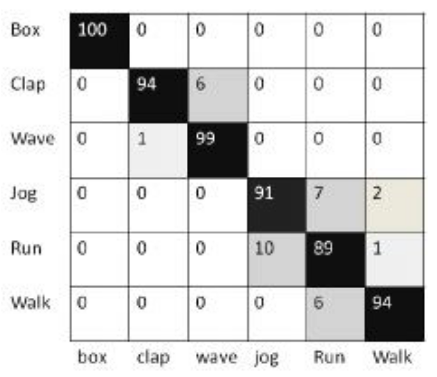
\includegraphics[width=0.6\linewidth]{imgs/chapter5/img6}
	\caption{Data features e attributi}
	\label{fig:chapter05-06}
\end{figure}

\section{Funzioni di split o routing}
Il routing o split $\phi\in\{L,R\}^{\mathcal{X}}$ determina se un data point $x\in\mathcal{X}$ deve muoversi a destra (i.e. $\phi(x)=\mathcal{R}$) o sinistra (i.e. $\phi(x)=\mathcal{L}$).
La possibile funzione di split \`e ristretta in un insieme predefinito $\Phi\subset\{L,R\}^\mathcal{X}$ in base alla natura dello spazio di features.
La funzione di split prototipica per un input $d$ dimensionale prima seleziona una dimensione e poi applica un criterio di split $1$ dimensionale.

	\subsection{Features discrete e nominali}
	Si assumano features discrete e nominali con valori in $\mathcal{K}$.
	La funzione di split pu\`o essere implementata data una partizione di $\mathcal{K}$ in $\mathcal{K}_R$ e $\mathcal{K}_L$:
	$$\phi(x) = \begin{cases}L &\mathbf{if} x\in\mathcal{K}_L\\
		R &\mathbf{if} x\in\mathcal{K}_R
	\end{cases}$$
	Trovare lo split ottimale richiede testare $2^{|\mathcal{K}|-1}-1$ bi-partizioni.
	
	\subsection{Features ordinali}
	Si assumano features ordinali con valori in $\mathcal{K}$.
	La funzione di split pu\`o essere implementata dando una soglia $r\in\mathcal{K}$:
	$$\phi(x) = \begin{cases}L &\mathbf{if} x\le r\\
		R &\mathbf{if} x>r
	\end{cases}$$
	Se $|\mathcal{K}|\le|\mathcal{D}|$ trovare lo split ottimale richiede il test di $|\mathcal{K}|-1$ soglie.
	Se $|\mathcal{K}|>|\mathcal{D}|$ si deve ordinare i valori di input in $\mathcal{D}$ dove $\mathcal{D}$ \`e il training set che raggiunge il nodo e testare $|\mathcal{D}|-1$ soglie.
	
	\subsection{Obliquo}
	A volte \`e conveniente fare split considerando pi\`u features alla volta.
	Tali funzioni lavorano con features continue e sono dette oblique in quanto generano decision boundaries obliqui.
	Se $x\in\mathbb{R}^d$ allora la funzione di split pu\`o essere implementata dato $w\in\mathbb{R}^d$ e $r\in\mathbb{R}$:
	$$\phi(x) = \begin{cases}L &\mathbf{if} w^Tx\le r\\
		R &\mathbf{altimenti}
	\end{cases}$$
	Si nota come questa funzione sia pi\`u difficile da ottimizzare.
	
	\section{Decision trees e overfitting}
	I decision trees sono modelli non parametrici con una struttura determinata dai dati.
	Per questo sono flessibili e possono facilmente fare fit sul training set, con un alto rischio di overfitting.
	Tecniche standard per migliorare la generalizzazione si applicano ai decision trees:
	\begin{multicols}{2}
		\begin{itemize}
			\item Early stopping.
			\item Regularization.
			\item Data augmentation.
			\item Complexity reduction.
			\item Ensembling.
		\end{itemize}
	\end{multicols}
	Una tecnica per ridurre la complessit\`a a posteriori \`e detta pruning.
	Se abbiamo un gran numero di attributi, possiamo trovare regolarità senza senso nei dati. 
	Oppure possiamo rimuovere anche gli attributi irrilevanti (processo manuale - non sempre possibile).

\section{Random forest}
Le random forest sono ensembles di decision trees \ref{fig:chapter05-08}.
Ogni albero \`e tipicamente trained con una versione bootstrapped del training set campionata con sostituzione.
Le funzioni di split sono ottimizzate su features campionate a caso o completamente a caso (extremely randomized trees).
Questo aiuta ad ottenere decision trees decorrelati.
La predizione finale della foresta \`e ottenuta facendo la media delle predizioni per ogni albero nell'ensemble $\mathcal{Q}=\{t_1,\dots,t_T\}$.
$$f_\mathcal{Q}(x)=\dfrac{1}{T}\sum\limits_{j=1}^Tf_t(x)$$

\begin{figure}
	\centering
	\begin{minipage}{.5\textwidth}
		\centering
		\includegraphics[width=1\linewidth]{imgs/chapter5/img7}
		\caption{Decision trees e overfitting. Aumentare il numero di nodi sui dati di training sembrava una buona idea quando non lo era sui dati di test.}
		\label{fig:chapter05-07}
	\end{minipage}%
	\begin{minipage}{.5\textwidth}
		\centering
		\includegraphics[width=1\linewidth]{imgs/chapter5/img8}
		\caption{Ensemble learning.}
		\label{fig:chapter05-08}
	\end{minipage}
\end{figure}

\section{Confronto con KNN}
Si nota come a differenza dei decision trees KNN non richiede nessun training, ma la classificazione \`e pi\`u veloce per i decision trees in quanto KNN per ogni esempio deve calcolare $k$ distanze.
A differenza di KNN che tratta tutte le features in maniera uguale i decision trees permettono una selezione delle features pi\`u importanti facendo scelte pesate.
